\section{改变抽样机制}
\label{sec:vr-change-mechanism}

前两节的方法都保持样本之间相互独立。独立有它的代价：$n$个独立均匀点可能挤在一处，也可能留下大片空白，每个区域分到多少样本完全由运气决定。本节放弃样本之间的独立，转而有计划地安排基础随机数：规定每个区域分到的点数，让点集整体上铺得均匀，或者让成对的输出朝相反或相同的方向变化。每个点的边缘分布仍然正确，所以估计仍然无偏；变化的是点与点之间的协方差。

\paragraph{把积分搬到单位立方体上}
设第~\ref{chap:sample-generation}章给出了一个可计算的生成映射$T:[0,1)^d\to\mathcal{X}$，使$\bm{U}\sim\operatorname{Unif}([0,1)^d)$时$T(\bm{U})\sim P$。记$F=f\circ T$，则
\begin{equation}
 I=\mathbb{E}_P[f(X)]=\int_{[0,1)^d}F(\bm{u})\,\mathrm{d}\bm{u} .
 \label{eq:vr-unit-cube}
\end{equation}
例如相关的高斯向量$\mathcal{N}(\bm{\mu},\bm{\Sigma})$可以取
\[
 T(\bm{u})=\bm{\mu}+\bm{L}\bigl(\Phi^{-1}(u_1),\dots,\Phi^{-1}(u_d)\bigr)^{\top} ,
\]
其中$\bm{L}$是协方差矩阵$\bm{\Sigma}$的Cholesky因子。点集的安排都在$\bm{u}$上进行，目标坐标之间的相关结构由$T$负责保留。这样，本节的方法只需要处理“单位立方体上的均匀点”这一种对象；代价是它们的效果取决于$F=f\circ T$的性质，而不仅是$f$的性质。

\subsection{分层采样}
\label{sec:vr-stratified}

用$8$个独立均匀点计算$\int_0^1\mathrm{e}^{u}\,\mathrm{d}u$，落在左半区间的点数服从$\operatorname{Bin}(8,1/2)$，有$7\%$的机会是$0$、$1$、$7$或$8$个。左半区间的函数值小、右半区间的大，点数的偶然多少直接变成估计的偏高或偏低。如果事先规定每个子区间各放几个点，这部分波动就消失了。

\begin{definition}[分层采样估计]
\label{def:vr-stratified}
把$\mathcal{X}$分成互不相交的集合$A_1,\dots,A_K$，称为层，设各层概率$p_k=P(A_k)>0$已知，并且能从条件分布$P(\cdot\mid A_k)$抽样。取正整数$n_1,\dots,n_K$，$\sum_kn_k=n$。各层内独立抽取$X_{k,1},\dots,X_{k,n_k}\sim P(\cdot\mid A_k)$，层间也相互独立。称
\begin{equation}
 \hat{I}^{\mathrm{st}}=\sum_{k=1}^{K}p_k\,\hat{\mu}_k,\qquad \hat{\mu}_k=\frac{1}{n_k}\sum_{i=1}^{n_k}f(X_{k,i})
 \label{eq:vr-stratified}
\end{equation}
为\term{分层采样}（stratified sampling）估计。
\end{definition}

记层内均值与层内方差为
\[
 \mu_k=\mathbb{E}[f(X)\mid X\in A_k],\qquad \sigma_k^2=\operatorname{Var}\bigl(f(X)\bigm|X\in A_k\bigr) .
\]

\begin{theorem}[分层估计的方差]
\label{thm:vr-stratified}
设$\mathbb{E}_P[f^2]<\infty$。则$\hat{I}^{\mathrm{st}}$无偏，且
\begin{equation}
 \operatorname{Var}\bigl(\hat{I}^{\mathrm{st}}\bigr)=\sum_{k=1}^{K}\frac{p_k^2\,\sigma_k^2}{n_k} .
 \label{eq:vr-stratified-variance}
\end{equation}
若按\term{比例分配}（proportional allocation）取$n_k=np_k$，则
\begin{equation}
 \operatorname{Var}\bigl(\hat{I}^{\mathrm{st}}\bigr)=\frac1n\sum_{k=1}^{K}p_k\sigma_k^2=\frac{\sigma^2}{n}-\frac1n\sum_{k=1}^{K}p_k(\mu_k-I)^2\leq\frac{\sigma^2}{n} .
 \label{eq:vr-proportional}
\end{equation}
\end{theorem}

\begin{proof}
由全概率公式，$\sum_kp_k\mu_k=I$；每个$\hat{\mu}_k$是$\mu_k$的无偏估计，所以$\hat{I}^{\mathrm{st}}$无偏。各层的样本相互独立，方差相加；$\hat{\mu}_k$的方差为$\sigma_k^2/n_k$，乘以系数的平方$p_k^2$即为第$k$层的贡献。

比例分配时代入$n_k=np_k$即得第一个等号。把层号$J$（$X\in A_J$）看成一个离散随机变量，由全方差公式，
\[
 \sigma^2=\mathbb{E}\bigl[\operatorname{Var}(f\mid J)\bigr]+\operatorname{Var}\bigl(\mathbb{E}[f\mid J]\bigr)=\sum_kp_k\sigma_k^2+\sum_kp_k(\mu_k-I)^2 ,
\]
移项得第二个等号。
\end{proof}

式~\eqref{eq:vr-proportional}说明比例分配的分层永远不比独立抽样差：它把总方差中的层间部分$\sum_kp_k(\mu_k-I)^2$整个去掉了。这一部分正是“各层分到多少点由运气决定”造成的波动。层分得越细、层均值差别越大，去掉的越多。

\paragraph{考虑波动与成本的分配}
比例分配没有利用各层的波动大小。设第$k$层每个样本的成本为$c_k$，总预算为$\sum_kc_kn_k=C$，在式~\eqref{eq:vr-stratified-variance}中选$n_k$。暂时允许$n_k$取正实数，由Cauchy--Schwarz不等式，
\[
 \Bigl(\sum_kp_k\sigma_k\sqrt{c_k}\Bigr)^2=\Bigl(\sum_k\frac{p_k\sigma_k}{\sqrt{n_k}}\cdot\sqrt{c_kn_k}\Bigr)^2\leq\Bigl(\sum_k\frac{p_k^2\sigma_k^2}{n_k}\Bigr)\Bigl(\sum_kc_kn_k\Bigr) .
\]
右边第二个因子是$C$，所以方差不小于$(\sum_kp_k\sigma_k\sqrt{c_k})^2/C$。等号当且仅当两个因子成比例，即
\begin{equation}
 n_k\propto\frac{p_k\sigma_k}{\sqrt{c_k}},\qquad \operatorname{Var}\bigl(\hat{I}^{\mathrm{st}}\bigr)_{\min}=\frac{\bigl(\sum_kp_k\sigma_k\sqrt{c_k}\bigr)^2}{C} .
 \label{eq:vr-neyman}
\end{equation}
波动大的层多放点，昂贵的层少放点。各层成本相同时$n_k\propto p_k\sigma_k$，称为\term{Neyman分配}（Neyman allocation）。实际的$n_k$要取整；若还要在层内估计方差，每层至少需要两个点。

\paragraph{例子：四层计算$\mathrm{e}-1$}
把$[0,1)$等分为四层，$p_k=1/4$。在宽为$1/4$的区间$[a,a+\tfrac14)$上，层均值与层内方差可以直接积分：
\[
 \mu_k=4\bigl(\mathrm{e}^{a+1/4}-\mathrm{e}^{a}\bigr),\qquad \sigma_k^2=2\bigl(\mathrm{e}^{2a+1/2}-\mathrm{e}^{2a}\bigr)-\mu_k^2 .
\]
四层的结果为
\[
 \begin{array}{lcccc}
  \text{层} & [0,\tfrac14) & [\tfrac14,\tfrac12) & [\tfrac12,\tfrac34) & [\tfrac34,1)\\
  \mu_k & 1.1361 & 1.4588 & 1.8731 & 2.4051\\
  \sigma_k & 0.0819 & 0.1052 & 0.1351 & 0.1735
 \end{array}
\]
取$n=8$，比例分配每层$2$个点，由式~\eqref{eq:vr-proportional}，
\[
 \operatorname{Var}\bigl(\hat{I}^{\mathrm{st}}\bigr)=\frac18\cdot\frac14\sum_k\sigma_k^2\approx0.002067 ,
\]
而$8$个独立点的方差为$0.24204/8\approx0.03025$，降为$1/14.6$。Neyman分配按$\sigma_k$的比例给出$n_k\approx1.32,1.70,2.18,2.80$，方差降到$0.001920$；取整为$1,2,2,3$时为$0.001963$，但第一层只有一个点，无法估计它的层内方差。这里各层波动相差不到三倍，最优分配只比比例分配好$7\%$。

下面用八个层内均匀数演示比例分配的计算，第$k$层的点取$u=(k-1+v)/4$：
\[
 v=0.37,\ 0.81\ \big|\ 0.06,\ 0.52\ \big|\ 0.23,\ 0.68\ \big|\ 0.45,\ 0.91 .
\]
得到的八个点依次为
\[
 u=0.0925,\ 0.2025,\ 0.265,\ 0.38,\ 0.5575,\ 0.67,\ 0.8625,\ 0.9775 .
\]
层均值的估计是每层两个$\mathrm{e}^{u}$的平均，再按$p_k=1/4$加权；因为比例分配，这等于八个函数值的普通平均：
\[
 \hat{I}^{\mathrm{st}}=\frac18\bigl(1.0969+1.2245+\cdots+2.6578\bigr)=1.7268 .
\]
真值为$1.7183$。

\begin{BookInlineFigure}
 \centering
 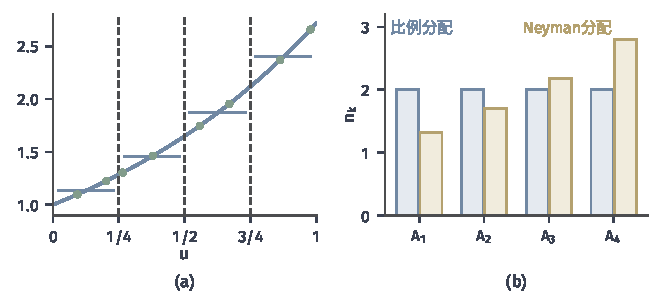
\includegraphics[width=112mm]{figures/07-probability/08-sampling-and-integration/matplotlib/vr-stratified/figure.pdf}
 \caption{四层分层采样计算$\int_0^1\mathrm{e}^{u}\,\mathrm{d}u$。(a)蓝线为$\mathrm{e}^{u}$，虚线为层的边界，蓝色短横线为层均值$\mu_k$，绿点为每层两个样本（$v$见正文）。(b)$n=8$时的样本分配：蓝色为比例分配$n_k=2$，黄色为Neyman分配$n_k\propto\sigma_k$。}
 \label{fig:vr-stratified}
\end{BookInlineFigure}

\paragraph{层越细越好，但维数会让层数爆炸}
图~\ref{fig:vr-stratified}(a)中，层内的函数几乎是直线，层内波动远小于整体波动。把$[0,1)$等分成$n$层、每层一个点，式~\eqref{eq:vr-stratified-variance}成为$n^{-2}\sum_k\sigma_k^2$。若$\lvert F'\rvert\leq L$，宽为$1/n$的层上$F$的取值范围不超过$L/n$，层内方差不超过$(L/n)^2/4$，于是
\[
 \operatorname{Var}\bigl(\hat{I}^{\mathrm{st}}\bigr)\leq\frac{1}{n^2}\cdot n\cdot\frac{L^2}{4n^2}=\frac{L^2}{4n^3} .
\]
方差按$n^{-3}$而非$n^{-1}$下降。到了$d$维，把每个坐标分成$m$段需要$m^d$个层，$d=10$、$m=2$就已经是$1024$层，每层至少一个点；预算不足$m^d$时，联合分层根本无法实施。

\paragraph{层的概率与分配不能由同一批数据随意决定}
定理~\ref{thm:vr-stratified}假设$p_k$已知、$n_k$事先固定。若$p_k$本身要从样本估计，估计量就变成两个随机量的组合，偏差和方差都要重新推导。若$n_k$按一次独立的试运行估计的$\sigma_k$确定，那么给定试运行结果，分配是固定的，定理的结论在条件意义下仍然成立；若边抽样边根据已抽到的值调整$n_k$，各层的样本数依赖于样本本身，式~\eqref{eq:vr-stratified-variance}不能直接套用，需要另行分析。

\subsection{拉丁超立方采样}
\label{sec:vr-lhs}

联合分层在高维失效，但退一步，可以只要求每个坐标各自分层：$n$个点投影到任何一根坐标轴上，都恰好在$n$个等长小区间中各占一个。这样，无论维数多大，$n$个点就够了。

\begin{definition}[拉丁超立方设计]
\label{def:vr-lhs}
给定点数$n$与维数$d$。取$d$个相互独立、在$\{1,\dots,n\}$的全部排列上均匀分布的随机排列$\pi_1,\dots,\pi_d$，再取与它们独立的$V_{i,j}\sim\operatorname{Unif}(0,1)$，$i=1,\dots,n$，$j=1,\dots,d$，全部相互独立。令
\begin{equation}
 U_{i,j}=\frac{\pi_j(i)-1+V_{i,j}}{n},\qquad \bm{U}_i=(U_{i,1},\dots,U_{i,d}) ,
 \label{eq:vr-lhs}
\end{equation}
用
\begin{equation}
 \hat{I}^{\mathrm{LHS}}=\frac1n\sum_{i=1}^{n}F(\bm{U}_i)
 \label{eq:vr-lhs-estimator}
\end{equation}
估计式~\eqref{eq:vr-unit-cube}的积分。
\end{definition}

第$i$个点的第$j$个坐标落在第$\pi_j(i)$层，层内位置由$V_{i,j}$决定。因为$\pi_j$是排列，第$j$个坐标的$n$个值恰好每层一个。这种设计称为拉丁超立方采样（Latin hypercube sampling，LHS），也叫\term{拉丁超立方抽样}。

\begin{theorem}[拉丁超立方的无偏性]
\label{thm:vr-lhs-unbiased}
在定义~\ref{def:vr-lhs}中，每个$\bm{U}_i$都服从$\operatorname{Unif}([0,1)^d)$。所以对可积的$F$，$\mathbb{E}[\hat{I}^{\mathrm{LHS}}]=I$。
\end{theorem}

\begin{proof}
固定$i$与$j$。均匀随机排列下$\pi_j(i)$在$\{1,\dots,n\}$上均匀分布，且与$V_{i,j}$独立。对$t\in[0,1]$，按层号分解，
\[
 \begin{aligned}
 \mathbb{P}(U_{i,j}\leq t)&=\sum_{k=1}^{n}\frac1n\,\mathbb{P}\Bigl(\frac{k-1+V_{i,j}}{n}\leq t\Bigr)\\
 &=\sum_{k=1}^{n}\frac1n\min\bigl\{1,\max\{0,nt-k+1\}\bigr\}=t .
 \end{aligned}
\]
最后一步中，$t$所在层之前的各层贡献$1/n$，$t$所在层贡献其中的一部分，之后的各层贡献$0$。不同的$j$用的是相互独立的$(\pi_j,V_{1,j},\dots,V_{n,j})$，所以$U_{i,1},\dots,U_{i,d}$相互独立，$\bm{U}_i$在立方体上均匀。对$n$个点的$F$值取期望并平均，得到无偏性。
\end{proof}

\paragraph{二维四点}
取$n=4$，$d=2$，两个排列与层内位置为
\[
 \pi_1=(2,4,1,3),\qquad \pi_2=(1,3,2,4) ,
\]
\[
 V_{:,1}=(0.37,0.81,0.06,0.52),\qquad V_{:,2}=(0.23,0.68,0.45,0.91) .
\]
由式~\eqref{eq:vr-lhs}，第一个点为
\[
 \bm{U}_1=\Bigl(\frac{1+0.37}{4},\ \frac{0+0.23}{4}\Bigr)=(0.3425,0.0575) .
\]
同样得到
\[
 \bm{U}_2=(0.9525,0.67),\qquad \bm{U}_3=(0.015,0.3625),\qquad \bm{U}_4=(0.63,0.9775) .
\]
图~\ref{fig:vr-lhs-points}(a)把单位正方形分成$4\times4$个格子：每行、每列恰好一个点，但$16$个格子只占了$4$个。逐维覆盖不等于覆盖全部坐标组合。图(b)是另一种同样合法的设计，两个排列都取恒等排列，四个点全落在对角线的格子里，坐标之间几乎完全相关。这种设计出现的概率是$1/4!$，它提醒我们：拉丁超立方只控制每个坐标的投影，不控制点在平面上的整体分布。

\begin{BookInlineFigure}
 \centering
 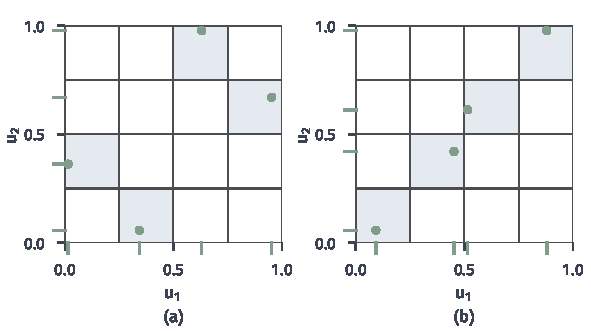
\includegraphics[width=100mm]{figures/07-probability/08-sampling-and-integration/matplotlib/vr-lhs-points/figure.pdf}
 \caption{$n=4$、$d=2$的拉丁超立方设计。灰线把正方形分成$4\times4$格，浅蓝格子含有一个点，坐标轴旁的绿色短线是点在各坐标上的投影。(a)$\pi_1=(2,4,1,3)$，$\pi_2=(1,3,2,4)$；(b)两个排列都是恒等排列。两者的$V$相同，见正文。}
 \label{fig:vr-lhs-points}
\end{BookInlineFigure}

对$F(\bm{u})=\mathrm{e}^{u_1}+\mathrm{e}^{u_2}$，真值$2(\mathrm{e}-1)=3.4366$。图(a)的四个点给出两列函数值的平均$1.7233$与$1.7770$，估计为$3.5004$。

\paragraph{可加函数：每个坐标都得到分层的好处}
先看$F$可以写成各坐标函数之和的情形。

\begin{theorem}[可加函数的拉丁超立方方差]
\label{thm:vr-lhs-additive}
设$F(\bm{u})=c+\sum_{j=1}^{d}g_j(u_j)$，各$g_j(U)$平方可积。记$\sigma_{j,k}^2$为$g_j(V)$在$V\sim\operatorname{Unif}([\tfrac{k-1}{n},\tfrac{k}{n}))$下的方差。则
\begin{equation}
 \operatorname{Var}\bigl(\hat{I}^{\mathrm{LHS}}\bigr)=\frac{1}{n^2}\sum_{j=1}^{d}\sum_{k=1}^{n}\sigma_{j,k}^2\leq\frac1n\sum_{j=1}^{d}\operatorname{Var}\bigl(g_j(U)\bigr) .
 \label{eq:vr-lhs-additive}
\end{equation}
\end{theorem}

\begin{proof}
估计量拆成$c+\sum_jT_j$，其中$T_j=\frac1n\sum_ig_j(U_{i,j})$只依赖第$j$列。第$j$列的$n$个值恰好每层一个，层内位置独立均匀，所以$T_j$正是每层一个点、$p_k=1/n$的分层估计，由式~\eqref{eq:vr-stratified-variance}，它的方差为$n^{-2}\sum_k\sigma_{j,k}^2$。不同列由相互独立的排列与层内位置生成，$T_1,\dots,T_d$相互独立，方差相加，得到等式。不等式是式~\eqref{eq:vr-proportional}对每一列的应用。
\end{proof}

对$F=\mathrm{e}^{u_1}+\mathrm{e}^{u_2}$，独立抽样的单点方差是$2\times0.24204$，而由上一小节的论证，式~\eqref{eq:vr-lhs-additive}按$n^{-3}$下降。图~\ref{fig:vr-lhs-variance}中绿线是比值$n\operatorname{Var}(\hat{I}^{\mathrm{LHS}})/\sigma^2$，它以$n^{-2}$的速度趋于零。

\paragraph{交互项：可能比独立抽样更差}
再看一个没有任何可加部分的函数。令$s(t)=1$（$t\geq\tfrac12$）或$-1$（$t<\tfrac12$），
\[
 F(\bm{u})=s(u_1)\,s(u_2) .
\]
$I=0$，$\sigma^2=1$，独立抽样的方差为$1/n$。设$n$为偶数，则第一个坐标落在下半区间$[0,\tfrac12)$的点恰有$n/2$个，第二个坐标也是。记$N$为两个坐标都在下半区间的点数。由$\pi_2$与$\pi_1$独立，第二个坐标落在下半区间的那些点是从$n$个点中均匀抽取的$n/2$个，所以$N$服从超几何分布$\operatorname{Hyp}(n,n/2,n/2)$。四类点的个数分别为
\[
 \text{下下}=N,\qquad \text{下上}=\text{上下}=\frac n2-N,\qquad \text{上上}=N .
\]

$F$在下下与上上处为$1$，其余为$-1$，于是
\[
 \hat{I}^{\mathrm{LHS}}=\frac{2N-2(n/2-N)}{n}=\frac{4N-n}{n} .
\]
由第~\ref{chap:common-distributions}章超几何分布的方差，
\[
 \operatorname{Var}(N)=\frac n2\cdot\frac12\cdot\frac12\cdot\frac{n-n/2}{n-1}=\frac{n^2}{16(n-1)} .
\]
所以
\begin{equation}
 \operatorname{Var}\bigl(\hat{I}^{\mathrm{LHS}}\bigr)=\frac{16}{n^2}\operatorname{Var}(N)=\frac{1}{n-1}>\frac1n .
 \label{eq:vr-lhs-interaction}
\end{equation}
$n=2$时方差为$1$，是独立抽样$1/2$的两倍：两点必然一个在左下或右上、另一个在相反的角，两个函数值相同，等于只抽了一个点。

\begin{BookInlineFigure}
 \centering
 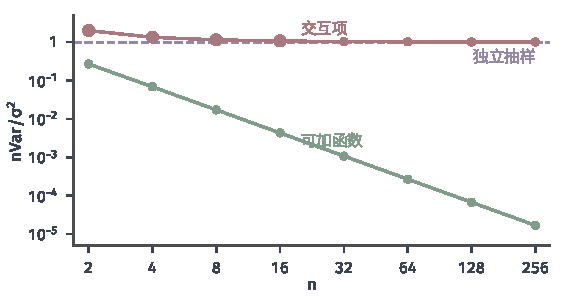
\includegraphics[width=96mm]{figures/07-probability/08-sampling-and-integration/matplotlib/vr-lhs-variance/figure.pdf}
 \caption{拉丁超立方的方差与独立抽样之比$n\operatorname{Var}(\hat{I}^{\mathrm{LHS}})/\sigma^2$，双对数坐标，$n$为偶数。绿线为可加函数$\mathrm{e}^{u_1}+\mathrm{e}^{u_2}$，按式~\eqref{eq:vr-lhs-additive}精确计算；红线为交互函数$s(u_1)s(u_2)$的精确值$n/(n-1)$，空心圆是$2\times10^{4}$次模拟（种子8）；紫色虚线为独立抽样。}
 \label{fig:vr-lhs-variance}
\end{BookInlineFigure}

\paragraph{一般函数}
一般的平方可积$F$可以分解为常数、各坐标的主效应$g_j(u_j)=\mathbb{E}[F(\bm{U})\mid U_j=u_j]-I$和剩下的交互部分。已知的结论是：拉丁超立方的方差等于$\sigma^2/n$减去$\frac1n\sum_j\operatorname{Var}(g_j(U_j))$，再加一个比$1/n$高阶的项；并且对任何平方可积的$F$和$n\geq2$，方差不超过$\sigma^2/(n-1)$。前者说明它去掉的正是主效应，后者说明它最多比独立抽样差一个因子$n/(n-1)$，式~\eqref{eq:vr-lhs-interaction}恰好达到这个上界。这两个结论的证明需要对排列做较长的组合计算，这里只用它们解释图~\ref{fig:vr-lhs-variance}：$F$越接近可加，拉丁超立方越有效；$F$以交互为主时，它几乎没有好处，有限样本下还可能略差。

\paragraph{误差怎样估计}
同一设计中的$n$个点不独立，它们的$F$值的样本方差除以$n$不是$\operatorname{Var}(\hat{I}^{\mathrm{LHS}})$的估计。正确的做法是第~\ref{chap:monte-carlo-integration-error}章的整组重复：独立生成$R$个设计，得到$R$个估计$Q_1,\dots,Q_R$，总平均$\bar{Q}$的方差用$s_Q^2/R$估计，$s_Q^2$是$Q_r$的样本方差。

\subsection{随机化准蒙特卡洛}
\label{sec:vr-rqmc}

分层与拉丁超立方都只控制点在若干固定格子中的个数。更直接的想法是：让点集在任何位置、任何尺度上都铺得均匀。先要有一个衡量“铺得均不均匀”的量。

对$\bm{b}\in[0,1]^d$，考虑以原点为一角的盒子$[\bm{0},\bm{b})=[0,b_1)\times\cdots\times[0,b_d)$。点集$\bm{a}_1,\dots,\bm{a}_n$均匀时，落进盒子的点的比例应当接近盒子的体积。

\begin{definition}[星差异]
\label{def:vr-star-discrepancy}
点集$\bm{a}_1,\dots,\bm{a}_n\in[0,1)^d$的\term{星差异}（star discrepancy）为
\begin{equation}
 D_n^{*}=\sup_{\bm{b}\in[0,1]^d}\Bigl\lvert\frac{\#\{i:\bm{a}_i\in[\bm{0},\bm{b})\}}{n}-\prod_{j=1}^{d}b_j\Bigr\rvert .
 \label{eq:vr-star-discrepancy}
\end{equation}
\end{definition}

一维时容易算。等距点$a_i=(i-1)/n$在$b$略大于$(i-1)/n$时，盒子里有$i$个点而长度只有约$(i-1)/n$，差$1/n$，所以$D_n^{*}=1/n$。把它们右移半格成$a_i=(i-\tfrac12)/n$，最大偏差减半为$1/(2n)$。$n=4$时，前者为$1/4$，后者为$1/8$。

图~\ref{fig:vr-discrepancy}比较了二维的两组$13$个点。独立均匀点（种子4）中，盒子$[0,0.607)\times[0,1)$的体积为$0.607$，却只含$3$个点，比例$0.231$，差$0.377$，这就是它的星差异。右图是一种规则构造：
\[
 \bm{a}_i=\Bigl(\frac{i-1}{13},\ \Bigl\{\frac{8(i-1)}{13}\Bigr\}\Bigr),\qquad i=1,\dots,13 ,
\]
其中$\{x\}=x-\lfloor x\rfloor$表示小数部分。它的星差异为$0.166$，由盒子$[0,0.538]\times[0,0.692]$达到：盒子连同边界上的点共$7$个，比例$0.538$，体积$0.373$。

\begin{BookInlineFigure}
 \centering
 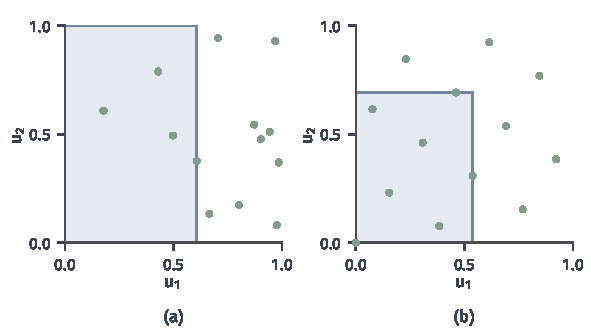
\includegraphics[width=100mm]{figures/07-probability/08-sampling-and-integration/matplotlib/vr-discrepancy/figure.pdf}
 \caption{$13$个点的星差异。浅蓝矩形是取到式~\eqref{eq:vr-star-discrepancy}中上确界的锚定盒子。(a)独立均匀点（种子4），盒子$[0,0.607)\times[0,1)$内只有$3$个点，$D_{13}^{*}=0.377$；(b)格点$((i-1)/13,\{8(i-1)/13\})$，盒子$[0,0.538]\times[0,0.692]$连同边界含$7$个点，$D_{13}^{*}=0.166$。}
 \label{fig:vr-discrepancy}
\end{BookInlineFigure}

\paragraph{确定性点集的积分误差}
用一个确定的点集代替随机样本，直接平均各点上的函数值，称为\term{准蒙特卡洛}（quasi-Monte Carlo）方法。它的误差由一个把函数与点集分开的不等式控制，称为\term{Koksma--Hlawka不等式}（Koksma--Hlawka inequality）：
\begin{equation}
 \Bigl\lvert\frac1n\sum_{i=1}^{n}F(\bm{a}_i)-\int_{[0,1)^d}F(\bm{u})\,\mathrm{d}\bm{u}\Bigr\rvert\leq V_{\mathrm{HK}}(F)\,D_n^{*} ,
 \label{eq:vr-koksma-hlawka}
\end{equation}
其中$V_{\mathrm{HK}}(F)$是$F$在Hardy--Krause意义下的变差，一维时就是$F$的全变差。证明需要多元的分部求和与变差的定义，篇幅较长。它的含义是：误差等于函数的起伏程度乘以点集的不均匀程度。一维的情形可以直接体会：$F$单调时，误差不超过$F$的总升降乘以$D_n^{*}$。

已有构造能使$D_n^{*}$随$n$按$(\ln n)^d/n$的阶下降，这样的点集称为\term{低差异点集}（low-discrepancy point set）；独立均匀点的星差异只按$n^{-1/2}$的阶下降。于是对$V_{\mathrm{HK}}(F)<\infty$的函数，准蒙特卡洛的误差在$n$很大时比$n^{-1/2}$小得多。但式~\eqref{eq:vr-koksma-hlawka}有三个局限：$V_{\mathrm{HK}}(F)$对无界函数和边界倾斜的示性函数是无穷；两个因子都难以计算，界本身不能用来报告误差；点集是确定的，算一次得到一个数，没有任何关于误差大小的信息。

\paragraph{加入随机性}
解决最后一个问题的办法是把整组点随机化：施加一个随机变换，使每个点单独看都服从均匀分布，而点集的均匀结构保持不变。这样得到的方法称为\term{随机化准蒙特卡洛}（randomized quasi-Monte Carlo，RQMC）。每个点均匀，保证估计无偏；整组独立重复若干次，就可以用第~\ref{chap:monte-carlo-integration-error}章的组间方差估计误差。下面讨论最简单的随机化，以及误差衰减的速度由什么决定。

\subsubsection{随机移位}
\label{sec:vr-random-shift}

把单位立方体的相对两面粘起来，它就成为一个环面：从右边出去的点从左边回来。在环面上整体平移一个点集，点与点之间的相对位置不变。

\begin{definition}[随机移位]
\label{def:vr-random-shift}
给定点集$\bm{a}_1,\dots,\bm{a}_n\in[0,1)^d$，取$\bm{\Delta}\sim\operatorname{Unif}([0,1)^d)$，令
\begin{equation}
 \bm{U}_i=(\bm{a}_i+\bm{\Delta})\bmod1,\qquad i=1,\dots,n ,
 \label{eq:vr-random-shift}
\end{equation}
其中$\bmod1$逐坐标取小数部分。所有点共用同一个$\bm{\Delta}$。称$Q=\frac1n\sum_iF(\bm{U}_i)$为\term{随机移位}（random shift）估计。
\end{definition}

例如$a=0.75$、$\Delta=0.37$时，$a+\Delta=1.12$，取小数部分得$0.12$：点从右端越过$1$后回到左端。图~\ref{fig:vr-random-shift}把上面的$13$点格点整体平移$\bm{\Delta}=(0.37,0.81)$：左图中平移后的点散在$[0,2)^2$的四块单位正方形里，右图把它们按$\bmod1$折回$[0,1)^2$，得到的仍是同一个格点结构，只是整体挪了位置。

\begin{BookInlineFigure}
 \centering
 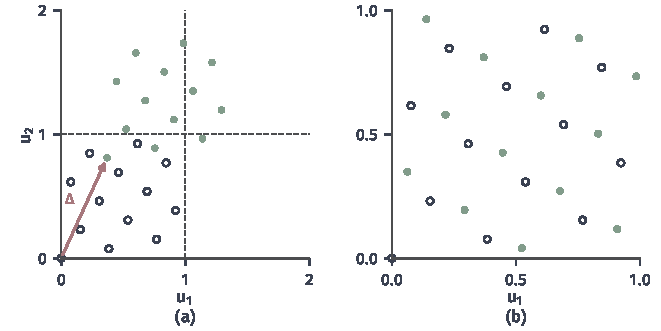
\includegraphics[width=112mm]{figures/07-probability/08-sampling-and-integration/matplotlib/vr-random-shift/figure.pdf}
 \caption{对$13$点格点的随机移位，$\bm{\Delta}=(0.37,0.81)$。空心圆为原格点，红色箭头为$\bm{\Delta}$。(a)平移后的点$\bm{a}_i+\bm{\Delta}$（绿色），虚线把$[0,2)^2$分成四块单位正方形；(b)逐坐标取小数部分后的$\bm{U}_i$（绿色）。}
 \label{fig:vr-random-shift}
\end{BookInlineFigure}

\begin{theorem}[随机移位的无偏性与方差]
\label{thm:vr-random-shift}
在定义~\ref{def:vr-random-shift}中，每个$\bm{U}_i$都服从$\operatorname{Unif}([0,1)^d)$，所以对可积的$F$，$\mathbb{E}[Q]=I$。若$F$平方可积，记其Fourier系数与点集的指数和为
\begin{equation}
 \begin{gathered}
 \hat{F}(\bm{h})=\int_{[0,1)^d}F(\bm{u})\mathrm{e}^{-2\pi\mathrm{i}\langle\bm{h},\bm{u}\rangle}\,\mathrm{d}\bm{u},\\
 S(\bm{h})=\frac1n\sum_{i=1}^{n}\mathrm{e}^{2\pi\mathrm{i}\langle\bm{h},\bm{a}_i\rangle},\qquad \bm{h}\in\mathbb{Z}^d ,
 \end{gathered}
 \label{eq:vr-fourier-sum}
\end{equation}
则
\begin{equation}
 \operatorname{Var}(Q)=\sum_{\bm{h}\neq\bm{0}}\bigl\lvert\hat{F}(\bm{h})\bigr\rvert^2\bigl\lvert S(\bm{h})\bigr\rvert^2 .
 \label{eq:vr-shift-variance}
\end{equation}
\end{theorem}

\begin{proof}
先证均匀性。一维时，固定$a\in[0,1)$，映射$\delta\mapsto(a+\delta)\bmod1$把$[0,1-a)$平移$a$得到$[a,1)$，把$[1-a,1)$平移$a-1$得到$[0,a)$，两段平移都保持长度，所以它把$[0,1)$上的均匀分布映成均匀分布。$d$维时$\bm{\Delta}$的各坐标独立，$\bm{U}_i$的各坐标也就独立且各自均匀。对$n$个点平均并取期望，得到无偏性。

再算方差。把$Q$看成$\bm{\Delta}$的函数：
\[
 Q(\bm{\Delta})=\frac1n\sum_{i=1}^{n}F\bigl((\bm{a}_i+\bm{\Delta})\bmod1\bigr) .
\]由平移保持均匀分布，每一项与$F$有相同的$L^2$范数，所以$Q$平方可积。

计算$Q$的Fourier系数时，对第$i$项作变量替换$\bm{v}=(\bm{a}_i+\bm{\Delta})\bmod1$，这一替换保持均匀测度。因为$\bm{h}$是整数向量，取小数部分不改变指数：
\[
 \mathrm{e}^{-2\pi\mathrm{i}\langle\bm{h},\bm{\Delta}\rangle}=\mathrm{e}^{-2\pi\mathrm{i}\langle\bm{h},\bm{v}\rangle}\,\mathrm{e}^{2\pi\mathrm{i}\langle\bm{h},\bm{a}_i\rangle} .
\]
于是
\[
 \hat{Q}(\bm{h})=\frac1n\sum_{i=1}^{n}\mathrm{e}^{2\pi\mathrm{i}\langle\bm{h},\bm{a}_i\rangle}\int_{[0,1)^d}F(\bm{v})\mathrm{e}^{-2\pi\mathrm{i}\langle\bm{h},\bm{v}\rangle}\,\mathrm{d}\bm{v}=\hat{F}(\bm{h})\,S(\bm{h}) .
\]

函数族$\mathrm{e}^{2\pi\mathrm{i}\langle\bm{h},\bm{u}\rangle}$（$\bm{h}\in\mathbb{Z}^d$）是$L^2([0,1)^d)$的完备正交规范系（可参考\BookChapterRef{chap:fourier-transform}{卷四第14章“Fourier变换”}），由Parseval等式（可参考\BookChapterRef{chap:function-inner-product-spaces}{卷四第12章“内积空间”}），
\[
 \mathbb{E}\bigl[\lvert Q\rvert^2\bigr]=\sum_{\bm{h}\in\mathbb{Z}^d}\bigl\lvert\hat{F}(\bm{h})S(\bm{h})\bigr\rvert^2 .
\]
$\bm{h}=\bm{0}$一项是$\lvert\hat{F}(\bm{0})\rvert^2=I^2$，因为$S(\bm{0})=1$。减去$I^2$即得式~\eqref{eq:vr-shift-variance}。
\end{proof}

\paragraph{点集是一个频率滤波器}
把式~\eqref{eq:vr-shift-variance}与独立抽样比较。对$F$本身用Parseval等式，
\[
 \sigma^2=\sum_{\bm{h}\neq\bm{0}}\bigl\lvert\hat{F}(\bm{h})\bigr\rvert^2 ,
\]
所以独立抽样的方差$\sigma^2/n$相当于给每个频率都乘上$1/n$。随机移位则给频率$\bm{h}$乘上$\lvert S(\bm{h})\rvert^2$。好的点集让$S(\bm{h})$在低频处为零或很小，只在少数高频处较大；只要$F$的能量主要集中在低频，方差就远小于$\sigma^2/n$。

格点是最干净的例子。取整数向量$\bm{z}$，令$\bm{a}_i=\{(i-1)\bm{z}/n\}$（逐坐标取小数部分）。$S(\bm{h})$是$n$个单位根的平均：若$\langle\bm{h},\bm{z}\rangle$是$n$的倍数，每项都是$1$，$S(\bm{h})=1$；否则$\mathrm{e}^{2\pi\mathrm{i}\langle\bm{h},\bm{z}\rangle/n}\neq1$，等比数列求和得$S(\bm{h})=0$。于是
\begin{equation}
 \operatorname{Var}(Q)=\sum_{\bm{h}\neq\bm{0},\ \langle\bm{h},\bm{z}\rangle\equiv0\ (\mathrm{mod}\ n)}\bigl\lvert\hat{F}(\bm{h})\bigr\rvert^2 .
 \label{eq:vr-lattice-variance}
\end{equation}
图~\ref{fig:vr-discrepancy}(b)的点集就是$n=13$、$\bm{z}=(1,8)$的格点，这类规则称为\term{秩1格点规则}（rank-1 lattice rule）。

\paragraph{一维等距点}
$d=1$、$z=1$时，$a_i=(i-1)/n$，只有$h$为$n$的倍数时$S(h)=1$，式~\eqref{eq:vr-lattice-variance}成为$\sum_{m\neq0}\lvert\hat{F}(mn)\rvert^2$。对$F(u)=\mathrm{e}^{u}$，
\[
 \hat{F}(h)=\int_0^1\mathrm{e}^{(1-2\pi\mathrm{i}h)u}\,\mathrm{d}u=\frac{\mathrm{e}-1}{1-2\pi\mathrm{i}h},\qquad \bigl\lvert\hat{F}(h)\bigr\rvert^2=\frac{(\mathrm{e}-1)^2}{1+4\pi^2h^2} .
\]
于是
\[
 \operatorname{Var}(Q)=2(\mathrm{e}-1)^2\sum_{m=1}^{\infty}\frac{1}{1+4\pi^2m^2n^2}\approx\frac{2(\mathrm{e}-1)^2}{4\pi^2n^2}\cdot\frac{\pi^2}{6}=\frac{(\mathrm{e}-1)^2}{12n^2} ,
\]
近似一步用了$\sum_m1/m^2=\pi^2/6$并略去分母中的$1$。均方根误差约为$0.496/n$，而独立抽样是$0.492/\sqrt{n}$。$n=4$时级数的精确值为$\operatorname{Var}(Q)=0.01536$，独立抽样为$0.06051$；$n=64$时分别为$6.01\times10^{-5}$与$3.78\times10^{-3}$。

\paragraph{整组重复估计误差}
取$n=4$的等距点$a=(0,\tfrac14,\tfrac12,\tfrac34)$，独立做$R=3$次随机移位。下面用三个移位量逐步演示：
\[
 \Delta=0.37,\quad 0.81,\quad 0.23 .
\]
第一次移位的点为$0.37,0.62,0.87,0.12$，其余两次分别为$0.81,0.06,0.31,0.56$与$0.23,0.48,0.73,0.98$。三组的估计为
\[
 Q_1=1.7053,\quad Q_2=1.6060,\quad Q_3=1.9036 .
\]
总平均$\bar{Q}=1.7383$，三个值的样本标准差$s_Q=0.1515$，标准误差估计为$s_Q/\sqrt3=0.0875$。按上面的精确方差，$\bar{Q}$的真实标准差是$\sqrt{0.01536/3}=0.0716$；同样$12$次求值的独立抽样标准差是$\sqrt{0.24204/12}=0.142$。三次重复给出的标准误差本身很粗糙；要构造第~\ref{chap:monte-carlo-integration-error}章的渐近误差区间，需要重复次数$R$趋于无穷，组内点数$n$固定时少量重复不能提供覆盖保证。同一组内的$4$个点不独立，不能用它们的样本方差除以$4$代替组间方差。

\subsubsection{误差衰减的条件}
\label{sec:vr-rqmc-rates}

随机移位对任何可积的$F$都无偏，但误差缩小得多快，由式~\eqref{eq:vr-shift-variance}决定：要看$F$的Fourier系数在$S(\bm{h})$较大的那些频率上衰减得多快。系数的衰减速度又由$F$在环面上的光滑程度决定，这里的“光滑”包括把立方体首尾粘起来以后的连续性。下面用一维等距点比较三种函数。

\paragraph{光滑但不周期}
$F(u)=\mathrm{e}^{u}$在$[0,1)$内光滑，但$F(0)=1\neq\mathrm{e}=F(1^{-})$，粘成圆周后在原点有一个跳跃。跳跃使$\hat{F}(h)$只按$1/\lvert h\rvert$衰减，上面已经算出均方根误差按$n^{-1}$下降。

\paragraph{换一个生成映射}
帐篷映射$\tau(u)=1-\lvert2u-1\rvert$把$\operatorname{Unif}(0,1)$映成$\operatorname{Unif}(0,1)$：对$t\in[0,1]$，$\tau(u)\leq t$当且仅当$u\leq t/2$或$u\geq1-t/2$，概率为$t$。所以$\widetilde{F}=F\circ\tau$与$F$的积分相同，单点方差也相同，只是换了一个生成映射。$\widetilde{F}(0)=\widetilde{F}(1^{-})=F(0)$，粘起来后连续，只在$u=\tfrac12$和原点处有折角，Fourier系数按$1/h^2$衰减，均方根误差按$n^{-2}$下降。

\paragraph{生成映射制造的奇异}
设目标是Pareto分布，$\mathbb{P}(X>x)=x^{-3}$（$x\geq1$），要算$\mathbb{E}[X]=3/2$。被积函数$f(x)=x$再光滑不过，但逆分位数映射$T(u)=(1-u)^{-1/3}$在$u\to1$时趋于无穷，于是
\[
 F(u)=f\bigl(T(u)\bigr)=(1-u)^{-1/3} .
\]
$\int_0^1(1-u)^{-2/3}\,\mathrm{d}u=3<\infty$，$F$平方可积，单点方差为$3-\tfrac94=\tfrac34$。但它在$u=1$处无界，$V_{\mathrm{HK}}(F)=\infty$，Koksma--Hlawka不等式失效。奇点$(1-u)^{-1/3}$使$\hat{F}(h)$只按$\lvert h\rvert^{-2/3}$衰减，于是方差按$\sum_m(mn)^{-4/3}\propto n^{-4/3}$下降，均方根误差按$n^{-2/3}$下降：仍比独立抽样快，但远慢于$\mathrm{e}^{u}$。

图~\ref{fig:vr-rqmc-rates}把三种情形与独立抽样画在一起，纵轴是均方根误差除以单点标准差。四条线的斜率依次接近$-\tfrac12$、$-\tfrac23$、$-1$、$-2$。同一个点集、同样的随机化，误差速度相差悬殊，差别全在$F=f\circ T$。

\begin{BookInlineFigure}
 \centering
 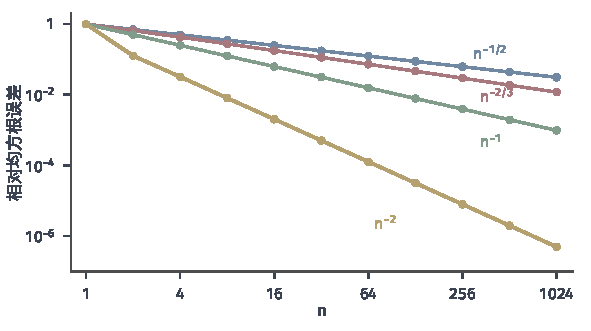
\includegraphics[width=100mm]{figures/07-probability/08-sampling-and-integration/matplotlib/vr-rqmc-rates/figure.pdf}
 \caption{一维等距点随机移位的相对均方根误差$\sqrt{\operatorname{Var}(Q)}/\sigma$，双对数坐标，由$\operatorname{Var}(Q)=n\int_0^{1/n}(Q(\Delta)-I)^2\,\mathrm{d}\Delta$数值积分得到。蓝线为独立抽样$n^{-1/2}$；绿线为$F(u)=\mathrm{e}^{u}$；黄线为帐篷映射后的$\mathrm{e}^{1-\lvert2u-1\rvert}$；红线为Pareto例子的$F(u)=(1-u)^{-1/3}$。}
 \label{fig:vr-rqmc-rates}
\end{BookInlineFigure}

\paragraph{点集与随机化方式}
高维时情况类似，但要同时看点集与随机化方式。格点配合随机移位，对在环面上光滑、Fourier系数衰减快的函数效果最好。另一大类低差异点集称为数字网，它的均匀结构是按二进制位定义的，普通的模$1$平移会破坏这种结构，需要配合按位的随机化，例如随机置乱。已知在被积函数足够光滑时，随机置乱的数字网的均方根误差可以接近$n^{-3/2}$的阶；这一结论的证明较长。无论哪种组合，更快的速度都只在相应的光滑条件下成立。

所以，不能只凭原函数$f$光滑，或者只凭点集差异小，就断言准蒙特卡洛会更准。要检查的是映射后的$F=f\circ T$：它在立方体边界上是否有界、粘起来后是否连续、是否有不沿坐标方向的间断。遇到不利的情形，可以像帐篷映射那样换一个生成映射，或者把奇异部分单独处理；无论效果如何，误差都用整组独立重复来估计。

\subsection{对偶变量}
\label{sec:vr-antithetic}

回到$\int_0^1\mathrm{e}^{u}\,\mathrm{d}u$。$U$与$1-U$都服从$\operatorname{Unif}(0,1)$，而且一个偏大时另一个必然偏小。把它们配成一对，$\mathrm{e}^{U}$偏高的那一次，$\mathrm{e}^{1-U}$就偏低，平均以后偏差部分抵消。

\begin{definition}[对偶变量估计]
\label{def:vr-antithetic}
设$n=2m$，$U_1,\dots,U_m$独立且都服从$\operatorname{Unif}(0,1)$。称
\begin{equation}
 \hat{I}^{\mathrm{anti}}=\frac1m\sum_{i=1}^{m}\frac{F(U_i)+F(1-U_i)}{2}
 \label{eq:vr-antithetic}
\end{equation}
为\term{对偶变量法}（antithetic variates）估计。它用了$n$次函数求值。
\end{definition}

每一对内两点的边缘分布都正确，所以估计无偏。记$\sigma^2=\operatorname{Var}(F(U))$，$\gamma=\operatorname{Cov}(F(U),F(1-U))$。一对的平均的方差为$(\sigma^2+\gamma)/2$，$m$对独立，所以
\begin{equation}
 \operatorname{Var}\bigl(\hat{I}^{\mathrm{anti}}\bigr)=\frac{\sigma^2+\gamma}{2m}=\frac{\sigma^2+\gamma}{n} .
 \label{eq:vr-antithetic-variance}
\end{equation}
同样$n$次求值的独立抽样方差是$\sigma^2/n$。两者相比，对偶变量严格更好当且仅当$\gamma<0$。

\begin{theorem}[单调函数的对偶协方差]
\label{thm:vr-antithetic-monotone}
设$F$在$(0,1)$上单调，$F(U)$平方可积。则$\operatorname{Cov}(F(U),F(1-U))\leq0$。
\end{theorem}

\begin{proof}
不妨设$F$不减。取与$U$独立同分布的$V$。若$U\geq V$，则$F(U)\geq F(V)$，同时$1-U\leq1-V$，$F(1-U)\leq F(1-V)$；$U<V$时两个不等号都反过来。所以
\[
 \bigl(F(U)-F(V)\bigr)\bigl(F(1-U)-F(1-V)\bigr)\leq0 .
\]
展开左边并取期望。由独立性与$1-V\sim\operatorname{Unif}(0,1)$，交叉项的期望都是$I^2$，于是期望等于$2\mathbb{E}[F(U)F(1-U)]-2I^2=2\gamma$，所以$\gamma\leq0$。
\end{proof}

\paragraph{例子与反例}
对$F(u)=\mathrm{e}^{u}$，$F(U)F(1-U)=\mathrm{e}$是常数，
\[
 \gamma=\mathrm{e}-(\mathrm{e}-1)^2\approx-0.23421 .
\]
由式~\eqref{eq:vr-antithetic-variance}，每次求值折合的方差为$\sigma^2+\gamma=0.24204-0.23421=0.00783$，相对效率约为$31$。用$u=0.37$与$0.81$各配一对：
\[
 \tfrac12(\mathrm{e}^{0.37}+\mathrm{e}^{0.63})=1.66267,\qquad \tfrac12(\mathrm{e}^{0.81}+\mathrm{e}^{0.19})=1.72858 ,
\]
平均$1.69563$。

反过来取关于$\tfrac12$对称的$F(u)=(u-\tfrac12)^2$，$I=1/12$。这时$F(1-U)=F(U)$，一对中的两个值完全相同，$\gamma=\sigma^2$，式~\eqref{eq:vr-antithetic-variance}给出$2\sigma^2/n$，是独立抽样的两倍：花了两次求值，只得到一个样本的信息。输入方向相反，本身不保证输出负相关。图~\ref{fig:vr-antithetic}对比了这两种情形。

\begin{BookInlineFigure}
 \centering
 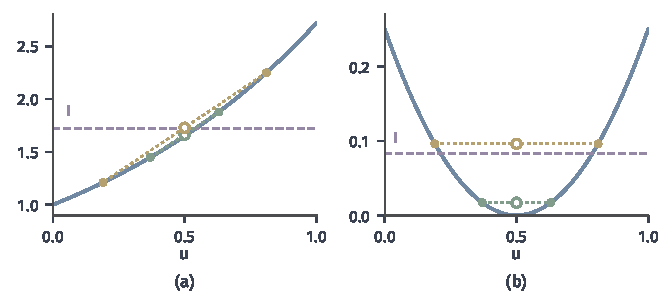
\includegraphics[width=112mm]{figures/07-probability/08-sampling-and-integration/matplotlib/vr-antithetic/figure.pdf}
 \caption{对偶对$(u,1-u)$，$u=0.37$（绿）与$u=0.81$（黄），实心点为两个函数值，$u=\tfrac12$处的空心圆为一对的平均，紫色虚线为积分值$I$。(a)单调的$\mathrm{e}^{u}$：一对的两个值分居$I$两侧，平均接近$I$；(b)对称的$(u-\tfrac12)^2$：一对的两个值相同，平均就是单个值。}
 \label{fig:vr-antithetic}
\end{BookInlineFigure}

\paragraph{奇偶分解}
两个例子可以统一起来。把$F$分成关于$\tfrac12$的偶部与奇部，
\[
 F_{\mathrm{e}}(u)=\frac{F(u)+F(1-u)}{2},\qquad F_{\mathrm{o}}(u)=\frac{F(u)-F(1-u)}{2} .
\]
一对的平均恰好是$F_{\mathrm{e}}(U)$，奇部被完全消去。$F_{\mathrm{e}}F_{\mathrm{o}}$关于$\tfrac12$是奇函数，积分为零，且$\mathbb{E}[F_{\mathrm{o}}(U)]=0$，所以$F_{\mathrm{e}}(U)$与$F_{\mathrm{o}}(U)$不相关，
\[
 \sigma^2=\operatorname{Var}\bigl(F_{\mathrm{e}}(U)\bigr)+\operatorname{Var}\bigl(F_{\mathrm{o}}(U)\bigr) .
\]
于是同样两次求值下，
\[
 \text{对偶一对的方差}=\operatorname{Var}(F_{\mathrm{e}}),\qquad \text{独立两点的方差}=\frac{\operatorname{Var}(F_{\mathrm{e}})+\operatorname{Var}(F_{\mathrm{o}})}{2} .
\]
对偶变量更好，当且仅当奇部的方差大于偶部的方差。单调函数以奇部为主，对称函数只有偶部。在$d$维中把$\bm{U}$换成$\bm{1}-\bm{U}$，对每个坐标都单调的$F$同样有$\gamma\leq0$，这一推广的证明要用到关于单调函数的关联不等式，篇幅较长；奇偶分解的判别对$d$维照样成立，论证与上面相同。

\subsection{共同随机数}
\label{sec:vr-crn}

另一类问题要比较两个方案。设方案A、B的输出分别为随机变量$A$与$B$，要估计期望差$\mathbb{E}[A]-\mathbb{E}[B]$。如果两个方案各自独立抽样，差的估计的方差是两者方差之和；但两个方案往往对同一种随机输入作出相似的反应，若让它们看到同一组随机输入，共同的波动就会在相减时抵消。

\paragraph{方差公式}
设$A=a(\bm{U})$，$B=b(\bm{U})$，$a(\bm{U})$与$b(\bm{U})$分别服从两个方案各自的输出分布。独立生成$\bm{U}_1,\dots,\bm{U}_n$，用
\[
 \hat{\Delta}=\frac1n\sum_{i=1}^{n}\bigl(a(\bm{U}_i)-b(\bm{U}_i)\bigr)
\]
估计$\mathbb{E}[A]-\mathbb{E}[B]$，这种做法称为\term{共同随机数}（common random numbers）。二阶矩有限时，
\begin{equation}
 n\operatorname{Var}(\hat{\Delta})=\operatorname{Var}(A)+\operatorname{Var}(B)-2\operatorname{Cov}(A,B) .
 \label{eq:vr-crn}
\end{equation}
两方案各用$n$个独立输入时，同样$2n$次求值得到的是$\operatorname{Var}(A)+\operatorname{Var}(B)$。所以$\operatorname{Cov}(A,B)>0$时共同随机数严格更好。若$a$与$b$都是同一个标量$U$的不减函数，重复定理~\ref{thm:vr-antithetic-monotone}的证明（这次两个因子同号），可得$\operatorname{Cov}(A,B)\geq0$。

这与对偶变量方向相反。对偶变量要估计一个量的平均，希望同一对中的两个输出负相关；共同随机数要估计两个量的差，希望两个输出正相关。

\paragraph{例子}
两个方案的输出是封顶为$1$的等待时间：$A=\min\{X_A,1\}$，$X_A\sim\operatorname{Exp}(1)$；$B=\min\{X_B,1\}$，$X_B\sim\operatorname{Exp}(1.25)$。都用逆分位数生成，$x=-\ln(1-u)/\lambda$。对非负变量，$\mathbb{E}[\min\{X,1\}]$等于$\mathbb{P}(X>t)$在$[0,1]$上的积分，所以
\[
 \mathbb{E}[A]=1-\mathrm{e}^{-1}=0.63212,\qquad \mathbb{E}[B]=\frac{1-\mathrm{e}^{-1.25}}{1.25}=0.57080 ,
\]
期望差为$0.06132$。数值积分给出$\operatorname{Var}(A)=0.12891$，$\operatorname{Var}(B)=0.12906$，用同一个$u$时$\operatorname{Cov}(A,B)=0.12707$。代入式~\eqref{eq:vr-crn}：
\[
 \begin{aligned}
 \operatorname{Var}(A)+\operatorname{Var}(B)&=0.25796,\\
 \operatorname{Var}(A-B)&=0.25796-2\times0.12707=0.003817 .
 \end{aligned}
\]
差的方差降为$1/67.6$。若不小心让B用$1-u$而A用$u$，两者变成负相关，$\operatorname{Var}(A-B)$升到$0.506$，比独立抽样还差一倍。图~\ref{fig:vr-crn}对比了独立输入与共同输入下的$(A,B)$。

\begin{BookInlineFigure}
 \centering
 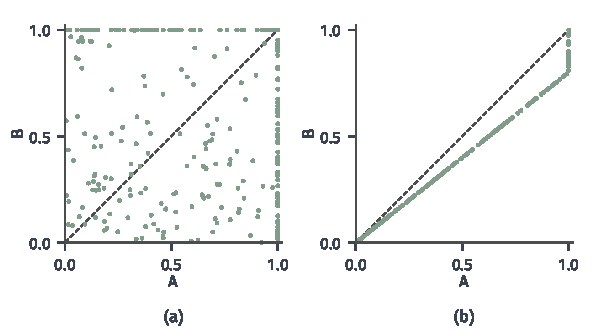
\includegraphics[width=100mm]{figures/07-probability/08-sampling-and-integration/matplotlib/vr-crn/figure.pdf}
 \caption{两个封顶等待时间$A=\min\{X_A,1\}$（$X_A\sim\operatorname{Exp}(1)$）与$B=\min\{X_B,1\}$（$X_B\sim\operatorname{Exp}(1.25)$）的$300$对样本（种子9），虚线为$A=B$。(a)两方案用独立的均匀数；(b)两方案用同一个均匀数，点落在一条递增曲线上，$A-B$的波动很小。}
 \label{fig:vr-crn}
\end{BookInlineFigure}

\paragraph{输入要按用途对齐}
复杂的模拟中，一次运行要消耗许多随机数。要让共同随机数起作用，两个方案应当在同样的用途上使用同一个随机数，例如第$k$个到达时刻都用第$k$个均匀数生成；若某个方案多消耗了一个随机数，后面的所有用途都会错位，协方差随之变小，甚至变号。

\paragraph{有限差分}
共同随机数的一个重要用途是用差商估计导数$\frac{\mathrm{d}}{\mathrm{d}\theta}\mathbb{E}[F(\theta,\bm{U})]$。两个参数值各用独立输入时，差商$\bigl(F(\theta+\delta,\bm{U})-F(\theta,\bm{U}')\bigr)/\delta$的方差约为$2\operatorname{Var}(F)/\delta^2$，$\delta$越小越糟；用同一个$\bm{U}$且$F$对$\theta$光滑时，分子约为$\delta\,\partial_\theta F(\theta,\bm{U})$，差商的方差保持有界。\BookChapterRef{chap:zeroth-order-optimization}{卷五第14章“零阶随机优化”}把这种做法称为共享样本，并分析了它在优化迭代中的作用；含参期望的导数怎样直接用样本表示，由第~\ref{chap:expectation-gradient-estimation}章研究。
